%%
% The BIThesis Template for Graduate Thesis
%
% Copyright 2020-2023 Yang Yating, BITNP
%
% This work may be distributed and/or modified under the
% conditions of the LaTeX Project Public License, either version 1.3
% of this license or (at your option) any later version.
% The latest version of this license is in
%   https://www.latex-project.org/lppl.txt
% and version 1.3 or later is part of all distributions of LaTeX
% version 2005/12/01 or later.
%
% This work has the LPPL maintenance status `maintained'.
%
% The Current Maintainer of this work is Feng Kaiyu.
\chapter{绪论 Introduction}

\label{chap:intro}
\section{研究的目的和意义 Purpose and Significance of This Research}

随着数字化、网络化、智能化技术的快速推进,全球网络空间正以前所未有的速度拓展,软件已渗透到政府管理、社会服务、产业控制、个人生活等各个层面。然而,软件的快速迭代与大规模部署在带来便利的同时,也使其成为网络攻击的重点目标。软件安全问题日益突出,恶意软件成为网络攻击中最活跃、最隐蔽、危害最大的武器之一,对国家安全、经济发展乃至社会稳定都构成了严重威胁。

With digitalization, networking, and artificial intelligence technologies developing rapidly, global cyberspace is expanding at an unprecedented pace. Software has permeated every layer of government administration, social services, industrial control, and personal life. However, the rapid iteration and large-scale deployment of software not only reveals that software brings convenience, but also implies that the software has also been a prime target for cyberattacks. Software security issues which pose a serious threat to national security, economic development, and even social stability have been more and more prominent, with the severe condition that malicious software emerges as one of weapons which is the most active, covert, and damaging in cyberattacks.

据《Security Navigator 2024》报告显示,2023年全球网络安全形势持续严峻,Orange Cyberdefense CyberSOC共检测129,395起网络攻击事件,同比增长30\%。其中,被安全分析师确认具有实际威胁的安全事件达25,076起,黑客攻击、权限滥用与恶意软件攻击占据主导地位。报告指出,2023年全球勒索软件受害者数量创下历史新高,同比激增46\%;政府机关、能源、电力、医疗等关键基础设施成为高级持续性威胁(APT)攻击的重点目标,呈现出“定向性强、潜伏时间长、破坏力大”的特点\cite{securitynavigator2024}。

The Security Navigator 2024 report reveals the fact that the global cybersecurity condition continued to be severe in 2023. Orange Cyberdefense's CyberSOC detected 129,395 cyberattack incidents, which represents an increase of 30\% compared to last year. Among these, security analysts confirmed 25,076 incidents that are dominated by hacker attacks, privilege abuse, and malicious software attacks result in actual threats. The report highlighted that the number of global ransomware victims reached a historic high in 2023, which surges 46\% compared to last year. Critical infrastructure sectors such as government agencies, energy, power, and healthcare became primary targets for Advanced Persistent Threat (APT) attacks, which are characterized as being highly targeted, long-dormant, and highly destructive.\cite{securitynavigator2024}

2025年2月,奇安信威胁情报中心发布的《网络安全威胁2024年度报告》分析了全球网络安全形势。2024年,APT攻击、勒索软件及黑灰产活动持续增长,多个恶意组织活跃,如Kimsuky、Lazarus等,频繁攻击关键软件系统和基础设施。此外,多个勒索组织间复杂的关联关系使得网络攻击更具隐蔽性和危害性,恶意软件的变种及漏洞利用愈发成为攻击的重要手段。报告还指出,银狐木马、Bigpanzi等黑灰产团伙对软件和网络安全构成了严重威胁,尤其是在软件漏洞利用和恶意代码传播方面\cite{qianxin2024}。

The Annual Cybersecurity Threat Report 2024, which is released by Qianxin Threat Intelligence Center, analyzed the global cybersecurity landscape in February 2025. In 2024, APT attacks, ransomware, and black-gray industry activities continued to increase. Multiple malicious groups such as Kimsuky and Lazarus persistently attacked critical software systems and infrastructure. In addition, intricate connections among ransomware groups made cyberattacks more covert and hazardous, while malware variants and vulnerability utilization increasingly became the key method of attack. The report also indicated that black-gray industry groups such as Silver Fox Trojan and Bigpanzi exposed severe threats to software security and network security, especially in the facet of software vulnerability utilization and malicious code propagation.

与此同时,攻击者手段不断演化,从早期的简单病毒、蠕虫程序逐步发展为以多阶段攻击链、自动化生成与逃逸机制为核心的智能恶意样本。特别是在AI技术支持下,恶意软件呈现“自学习、自适应、自变异”的智能特征,使得传统安全检测手段,如特征码比对、规则匹配、静态扫描等方式效果日益下降\cite{chen2018study, ren2021matching, lipp2022empirical}。据统计,现有静态检测技术对新型恶意样本的检测率已降至60\%以下,而通过简单扰动生成的对抗样本可使主流检测模型的误报率提升至80\%以上,暴露出当前检测体系在应对智能对抗方面的巨大短板。

Meanwhile, attacker tactics have consistently evolved from early simple viruses and worms to intelligent malicious samples which focus on multi-stage attacking chains, automated generation, and evasion mechanisms. Especially with the support of AI technologies, malicious software exhibits "self-learning, self-adaptation, and self-mutation" intelligent features, which make traditional malware detection methods—such as trait comparison, rule matching, and static scanning—increasingly ineffective\cite{chen2018study, ren2021matching, lipp2022empirical}. According to statistics, the detection rate of existing static techniques for novel malicious samples has dropped below 60\%, while adversarial samples which are generated from benign software by simple disturbances can increase the false positive rate of major popular detection models to over 80\%. This phenomenon exposes tremendous deficiencies in current malware detection systems against intelligent adversarial threats.

面对这种攻防失衡的格局,研究者们开始尝试采用强化学习等人工智能技术模拟攻击者视角,通过生成对抗样本促进检测系统的鲁棒性提升。然而,当前大多数对抗样本生成方法仍存在明显局限,如仅针对特定检测模型、扰动方式单一、未能充分考虑样本语义一致性与行为隐蔽性等,难以真实模拟复杂攻击场景中的“动态对抗过程”\cite{yu2022natural, ilahi2021challenges, labaca2021aimed,standen2025adversarial}。此外,现有方法对扰动成本与样本迁移能力考虑不足,导致生成样本难以推广应用,实用性不强。

Faced with this imbalance between attack and defense, researchers have begun to simulate attacker perspectives by artificial intelligence techniques like reinforcement learning, generating adversarial samples to enhance detection system robustness. However, most current adversarial generation methods still exist notable limitations, such as targeting only specific detection models, employing simplistic disturbance methods, and inadequately considering sample semantic consistency and behavioral concealment, which makes researchers fail to simulate "dynamic adversarial processes" in complex attack scenarios\cite{yu2022natural, ilahi2021challenges, labaca2021aimed,standen2025adversarial}. Moreover, existing methods are insufficient in the consideration of disturbances costs and sample transferability, which hinders the application, scalability, and practicality of generated samples.

因此,本研究在如此复杂严峻的网络安全背景下提出并构建一种基于强化学习的多维度对抗性恶意软件生成框架,具有突出的现实必要性与战略价值。该框架从软件的结构层、指令层和行为层三个维度进行扰动建模,并引入良性样本字节信息构建高隐蔽性扰动策略;采用PPO+LSTM的智能体设计,强化对扰动序列之间逻辑与语义关联的学习能力,提升逃避检测的有效性与生成样本的泛化能力。同时结合扰动成本与训练效率,设计动态奖励机制,以实现兼具实效性与性能的对抗样本生成。本研究不仅有助于揭示智能化攻击技术演化的规律与机制,提升对抗样本的真实性与适应性,还能作为新一代恶意软件检测系统的训练与评估工具,促进检测技术的迭代优化。更重要的是,它为构建“以攻促防”的智能安全生态体系提供了坚实支撑,在国家网络安全战略与实战攻防需求下具有显著的理论意义与应用前景。

Thus, this study proposes and constructs a multi-dimensional adversarial malware generation framework based on reinforcement learning, which has outstanding real necessities and strategic value in the background of complex and severe cybersecurity challenges. The framework builds disturbance modules through three dimensions of software—structural, instruction, and behavioral layers—and adopts benign sample bytes to craft highly concealed disturbance strategies. By employing an agent design based on PPO and LSTM, this framework enhances the learning ability of logical and semantic relations of disturbance sequences, which improves evasion detection effectiveness and the versatility of generated samples. Meanwhile, by combining disturbance cost and training efficiency, and designing a dynamic reward mechanism, this framework achieves the goal that it can generate adversarial samples which not only are effective but also have high performance.This research not only is helpful to reveal the evolutionary patterns and mechanisms of intelligent attack technologies, improving the reality and adaptability of generated adversarial samples, but also builds a tool for new generation malware detection systems training and evaluating, which fosters the iteration and optimization of malware detection techniques. Furthermore, this research provides robust support for establishing an intelligent "attack promotes defense" security ecosystem, which has significant theoretical significance and application prospects for national cybersecurity strategies and real attack-defense requirements.

\section{国内外研究现状 Current Domestic and International Research Condition }
%\label{sec:***} 可标注label
近年来,随着深度学习技术在图像识别、语音处理、自然语言理解、恶意代码检测等领域的广泛应用\cite{meng2022adavit,yang2022torchaudio,weld2022survey,lee2023classification},基于神经网络的智能系统在精度和效率上取得了突破性进展。然而,深度学习模型对输入数据的高度依赖性也暴露出其在安全性和鲁棒性方面的显著短板。

In recent years, with the extensive application of deep learning technology in realms such as image recognition\cite{meng2022adavit,yang2022torchaudio,weld2022survey,lee2023classification}, voice processing, natural language understanding, and malware detection, intelligent systems based on neural networks have achieved breakthroughs in accuracy and efficiency. However, deep learning models’ high dependency on input data also exposes significant absence in their security and robustness.

自2013年研究者首次提出“对抗样本”概念以来\cite{goodfellow2014explaining},该问题逐渐成为人工智能安全领域的核心议题。研究表明,深度神经网络对输入扰动极为敏感,即便是在原始输入中仅加入微小、肉眼难以察觉的扰动,也可能导致模型产生完全错误的输出。这类经过特定设计的扰动样本被称为“对抗样本”,其攻击方式被称为“对抗攻击”。

Since the concept of "adversarial examples" was first raised by researchers in 2013\cite{goodfellow2014explaining}, this issue has gradually become a central topic in artificial intelligence security. Studies reveal that deep neural networks are extremely sensitive to input disturbance; even adding subtle disturbance which can not be observed by human eyes to original inputs can cause models to produce completely erroneous outputs. These samples which are crafted deliberately to disturb are called "adversarial examples", whose attack methods are called "adversarial attacks".

针对这一问题,学术界和工业界相继提出了多种对抗样本生成方法,形成了较为系统的研究体系,基本模式如图\ref{fig:diagram}所示。现有对抗样本生成方法主要包括:

To solve this challenge, academic realms and industrial realms have proposed various adversarial example generation methods, forming a relatively systematic research framework, whose basic pattern is shown in figure \ref{fig:diagram}. Current adversarial generation methods mainly include:

\begin{figure}[hbt]
	\centering
	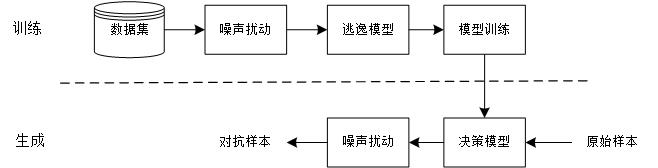
\includegraphics[width=0.75\textwidth]{figures/1.1}
	% \caption[这里的文字将会显示在 listoffigure 中]{这里的文字将会显示在正文中}
	\caption{对抗样本生成基本框架}\label{fig:diagram}
\end{figure}

\begin{enumerate} [label=\arabic*)] 
\item 基于梯度的攻击方法:如FGSM\cite{lupart2023study}(Fast Gradient Sign Method)、BIM\cite{kurakin2016adversarial}(Basic Iterative Method)、PGD\cite{bryniarski2021evading}(Projected Gradient Descent)等,通过利用模型的梯度信息快速生成对抗扰动。这类方法执行效率高,易于实现,广泛用于对抗训练。

Attack Methods Based on Gradient: such as FGSM\cite{lupart2023study} (Fast Gradient Sign Method), BIM\cite{kurakin2016adversarial} (Basic Iterative Method), and PGD\cite{bryniarski2021evading} (Projected Gradient Descent), which generate adversarial disturbance rapidly by utilizing model gradient information. These methods are efficient and easy to implement and are widely used in adversarial sample training.
\item 优化目标驱动方法:如C\&W攻击\cite{carlini2017towards}、DeepFool\cite{moosavi2016deepfool}等,通过构建特定的优化目标函数,最小化扰动幅度同时最大化模型输出的误导性,提高攻击的隐蔽性和精度。

Optimization Objective Driver Methods: such as C\&W attacks\cite{carlini2017towards} and DeepFool\cite{moosavi2016deepfool}, which construct functions optimizing objects to minimize disturbance magnitudes while misleading model maximally, enhancing attack concealment and precision.
\item 迁移型与黑盒攻击方法:此类方法在未知模型结构的情况下依然能实现攻击目标,如使用替代模型生成具有迁移能力的对抗样本,或基于查询机制的无梯度攻击方法,如NES攻击\cite{ilyas2017query}、ZOO攻击\cite{chen2017zoo}等。

Attack Methods Based on Transferability and Black Box: These methods can achieve attack goals without knowing the details of target model’s architecture, such as using transferable adversarial examples generated by alternative models, gradient-free attacks methods based on query mechanisms like NES attacks\cite{ilyas2017query} and ZOO attacks\cite{chen2017zoo}.
\item 对抗样本在安全领域的扩展应用:研究者逐渐将对抗样本技术拓展至文本、音频和恶意代码等复杂数据领域。在恶意软件检测任务中,对抗样本不仅需要误导分类器,更需保持原始代码功能的完整性,这对样本生成算法提出更高要求。

Extensive Applications of Adversarial Examples in Security: Researchers are increasingly extending adversarial example techniques to complex data realms like text, audio, and malicious code. In malware detection tasks, adversarial examples are required to not only mislead classifiers but also preserve the original code’s functional integrity, imposing higher requirements on sample generation algorithms.
\end{enumerate}

Kolosnjaji 等人\cite{kolosnjaji2018adversarial}提出了一种基于梯度的对抗攻击方法,仅修改恶意样本末尾少量字节即可成功绕过以原始字节为输入的深度恶意软件检测模型,且不影响其功能,揭示了此类模型在静态检测场景下的对抗脆弱性。

Kolosnjaji et al.\cite{kolosnjaji2018adversarial} proposed an adversarial attack method based on gradient, which successfully evades malware detection models based on deep learning and taking raw bytes as input by modifying only a few bytes at the end of malicious samples, without influencing their functionality, exposing the limitation of such models in static malware detection scenarios.

Hu和Tan等人在2022年提出了MalGAN\cite{hu2022generating},一种基于生成对抗网络(GAN)的黑盒对抗样本生成方法,用于攻击机器学习恶意软件检测系统。该方法通过训练一个生成器网络,使其生成能够绕过黑盒检测模型的对抗性恶意样本。

Hu and Tan et al. proposed MalGAN\cite{hu2022generating}, a black-box adversarial example generation method based on generating adversarial network (GAN) for attacking malware detection systems based on machine learning in 2022. This method trains a generator network to produce adversarial malware samples that can evade black-box detection models.

Grosse 等人(2017)\cite{grosse2017adversarial}将对抗样本攻击扩展至恶意软件检测领域,提出了一种改进的对抗样本生成方法,可在离散和二值输入空间中生成保持恶意功能的对抗样本。

In 2017, Grosse et al. extended adversarial sample attacks to malware detection realm\cite{grosse2017adversarial}, proposing an advanced adversarial sample generation method that creates adversarial samples that keep malicious functions in discrete and binary input spaces.

Demetrio等人在2019年探讨了卷积神经网络(CNN)在恶意软件检测中的对抗鲁棒性问题\cite{demetrio2019explaining}。研究发现,一些原本在图像分类中有效的攻击方法在恶意软件检测中失效,而 CNN 架构本身也存在特定弱点,可被利用设计新的攻击方式。

Demetrio et al. explored the adversarial robustness of convolutional neural networks (CNNs) in malware detection in 2019\cite{demetrio2019explaining}. Their study found that some origin effective attack methods for image classification failed in malware detection, while the CNN framework itself existed specific weaknesses that can be used to design new attack methods.

近年来,部分研究尝试将强化学习与对抗样本生成结合,建模为一个序列决策过程,使攻击策略更加智能化。

Recently, some studies have attempted to combine reinforcement learning and adversarial example generation, modeling it as a sequential decision process that makes attack strategies more intelligent.

Song等人提出了一种基于强化学习的纯黑盒对抗攻击框架\cite{song2022mab},用于生成针对 PE 恶意样本检测器和商业杀毒引擎的对抗样本。该方法将攻击过程建模为多臂老虎机问题,在探索和利用之间寻求最优平衡。Labaca-Castro等人提出AIMED-RL框架\cite{labaca2021aimed},该方法基于分布式双重 DQN,能够在不破坏恶意样本功能的前提下,通过强化学习自动生成对抗样本,实现对恶意软件分类模型的规避。Zhong等人提出了一个基于强化学习的框架\cite{zhong2022reinforcement},用于生成强对抗性的恶意软件样本,以逃避第三方检测器。该方法通过动态规划或时序差分学习自适应地选择最优扰动路径,该路径由Obfusmal、Stealmal和Hollowmal三种扰动方法组合而成。Homayoun等人提出了一种面向硬件恶意软件检测(HMD)系统的多阶段对抗性学习与防御框架\cite{he2024beyond}。该方法针对处理器性能计数器等结构化表格数据,在第一阶段使用有效对抗攻击规避机器学习检测;随后引入基于 Advantage Actor Critic(A2C)的深度强化学习方法实时预测攻击模式,并结合对抗训练增强模型鲁棒性。Li等人\cite{ebrahimi2022adversarial}针对基于机器学习的恶意软件检测器在对抗样本下鲁棒性不足的问题,提出了一种基于对抗最小最大优化的对抗学习框架。该方法将通过强化学习生成的对抗样本引入训练过程,通过攻击策略与检测模型的交替优化提升鲁棒性。

Song et al. proposed a purely black-box adversarial attack framework based on reinforcement learning for generating adversarial samples against PE malware detectors and commercial antivirus engines\cite{song2022mab}. This method models the attack process as a multi-armed bandit problem, finding an optimal balance between exploring and utilizing. Labaca-Castro et al. proposed the AIMED-RL framework based on distributed double DQN\cite{labaca2021aimed}, which could automatically generate adversarial samples by using reinforcement learning to evade malware classification models. Besides, the functions of malicious samplew are not broken. Zhong et al. raised a framework based on reinforcement learning which could be used to generate highly adversarial malware samples to evade third-party malware detectors\cite{zhong2022reinforcement}. This method uses dynamic programming or temporal difference learning to adaptively select optimal disturbance paths that incorporate Obfusmal, Stealmal, and Hollowmal three disturbance methods. Homayoun et al. raised a multi-stage adversarial learning and defense framework targeting hardware malware detection (HMD) systems\cite{he2024beyond}. This method targets structured tabular data, such as processor performance counters. In the first stage, it evades malware detection by using effective adversarial attacks, then introduces a deep reinforcement learning approach based on Advantage Actor Critic (A2C) to forecast attack patterns and integrates adversarial training methods to enhance model robustness. Li et al. addressed the issue that malware detectors based on machine learning robustness are insufficient against adversarial examples\cite{ebrahimi2022adversarial}, then offered an adversarial learning framework based on adversarial maximum and minimum optimization. This method integrates adversarial samples generated by reinforcement learning into training processes, alternately enhancing robustness by optimizing attack strategies and malware detection models.

尽管已有多种方法取得显著成果,但当前研究仍面临若干挑战。一方面,部分方法过于依赖模型结构或梯度信息,难以适应真实环境中的黑盒场景;另一方面,对抗样本在保证误导性的同时,往往牺牲了样本的可执行性或语义合理性,特别是在代码和文本等高语义数据上。此外,现有研究普遍侧重于攻击单一模型,对于联合防御、多模型集成系统的逃逸效果有限。

Although various methods get significant achievements, current research still faces several challenges. On the one hand, some methods rely excessively on model structure or gradient information, which makes them struggle to adapt to real black-box scenarios. On the other hand, while ensuring misguidance, adversarial examples often reduce sample executability or semantic plausibility, particularly for data that has highly semantic meaning, such as code and text. Furthermore, existing studies generally focus on attacking single models, limiting evasion effects against joint defense or multi-model integrated malware detection systems.

因此,如何在保证样本功能完整与语义一致的前提下,实现对多种检测系统的有效攻击,成为当前研究的重要方向。同时,如何设计通用、轻量、高迁移性的攻击框架,也成为未来研究的关键课题。

Therefore, how to effectively attack multiple detection systems while ensuring sample functional integrity and semantic consistency has become a crucial research direction of current research. Meanwhile, designing universal, light, and highly transferable attack frameworks is also a key challenge for future research.

\section{本文研究内容 Research Content of This Paper}
%\label{sec:features}

本文围绕“基于强化学习的多维度对抗性恶意软件生成方法”展开,旨在突破当前对抗样本生成方法在模型迁移性、扰动精细性及逃逸能力等方面的瓶颈,构建一个具备实用性和泛化性的智能对抗框架。具体研究内容如下:

This study focuses on the "reinforcement learning-based multi-dimensional adversarial malware generation method" and aims to overcome the difficulties of adversarial sample generation methods, such as model transferability, disturbance accuracy, and evasion capability by constructing an intelligent adversarial framework with practicality and versatility. The specific research contents are listed as follows:
\begin{enumerate} [label=\arabic*)] 
\item 恶意软件扰动维度建模与设计。针对传统对抗性样本生成方法多以字节插入、节区填充等静态操作为主,缺乏对样本行为层面的深入干预,本文从结构层、指令层与行为层三个维度对原始恶意样本进行扰动建模,系统构建了可控的扰动操作空间。结构层扰动包括节区重命名、节区重排序、空节填充等对样本格式产生改变但不影响可执行性的操作;指令层扰动主要包括无操作指令插入、等价指令替换等轻量级代码层扰动;行为层扰动涉及系统调用替换、配置路径扰动等对动态行为产生微妙变异的操作。这一多维设计旨在提升扰动的多样性与组合能力,为后续的策略学习提供丰富操作选择。

Malware Disturbance Dimension Modeling and Design: To solve the limitation that traditional adversarial sample generation methods mainly rely on static operations that are insufficient for having intervention at the behavioral layer of samples such as byte insertion or section padding, this research models disturbance of original malware from three dimensions—structural layer, instruction layer, and behavioral layer, systematically establishing a controllable disturbance operation space. Structural layer disturbance includes operations that modify sample format without affecting executability, such as section renaming, section resorting, and section padding. Instruction layer disturbance mainly contains slight code level operations like inserting no-operation (NOP) instructions or replacing equivalent instructions. Behavioral layer disturbance is comprised by operations that subtly modify malware dynamic behavior, such as replacing system calls or disturbing configuration paths. This multi-dimensional design aims to enhance disturbance diversity and combining abilities, providing abundant operational choices for following strategy learning.
\item 引入良性样本特征扰动机制。有别于传统使用随机扰动或无效填充字节的方式,本文创新性地引入真实良性软件样本中的特征字节序列作为扰动来源,增强对抗样本的“良性掩盖效应”,提高检测系统误判率。通过构建良性字节库,并对其语义信息进行编码与筛选,在扰动过程中优先选取与目标样本语义接近的良性片段嵌入,使生成样本更具可解释性和混淆性。

Introducing Benign Sample Feature Disturbance Mechanism: Different from traditional methods using random noise or invalid padding bytes, this study innovatively introduces feature byte sequences that are extracted from real benign software samples as disturbance byte sources. This method enhances the "benign concealment effect" of adversarial samples and increases the misjudgment rate of malware detection systems. By constructing a benign byte repository and through encoding and filtering its semantic information, it prioritizes selecting benign fragments similar to the target sample to embed in the target sample during disturbance, which improves the interpretability and obfuscation capability of generated samples.
\item 强化学习环境建模与策略优化方法设计。本文将对抗样本生成过程建模为强化学习中的序列决策问题。状态空间定义为当前恶意样本的扰动历史与静态/动态特征;动作空间为预定义的扰动操作集;奖励函数综合考虑逃逸成功率、扰动成本、执行有效性等多维度指标。为增强序列建模能力,本文引入长短期记忆网络(LSTM)结构,作为策略网络的一部分,建模扰动序列间的时间依赖关系。同时,使用PPO(Proximal Policy Optimization)算法提升策略学习的稳定性和训练效率,缓解强化学习在高维稀疏奖励场景下的训练困难。

Reinforcement Learning Environment Modeling and Strategy Optimization Design: This research regards the adversarial sample generation process as a sequential problem about making decisions in reinforcement learning. The state space is defined as the disturbance history, static features, and dynamic features of the current malware sample. The action space is composed of the predefined disturbance operation set. The reward function considers multiple dimensions indicators such as evasion success rate, disturbance cost, and execution effectiveness. To enhance sequential modeling ability, a Long Short-Term Memory (LSTM) network is introduced as a section of the policy network to model the temporal dependencies between perturbation sequences. Besides, the Proximal Policy Optimization (PPO) algorithm is being used to improve the stability and training efficiency of strategy learning, which alleviates the training difficulties in high dimensional sparse reward scenarios.
\item 动态奖励机制设计与泛化能力优化。为提高生成样本的实用性与跨平台攻击能力,本文设计了一个基于目标检测器反馈与扰动代价联合驱动的动态奖励函数,以实现对训练资源和扰动成本的双重约束。		

Dynamic Reward Mechanism Design and Generalization Ability Optimization: To enhance the generated sample practicality and make the generated sample have the ability to attack multiple platforms, this research designs a dynamic reward function driven by target detector feedback and disturbance cost to constrain training resources and disturbance cost.
\end{enumerate}

此外,本文引入多个异构检测器构建多模型训练环境,提升策略泛化能力,使生成的样本不仅能成功绕过训练时的目标模型,还具备较强的迁移性,能够对抗未知或演化型检测系统。

Furthermore, multiple heterogeneous detectors are introduced to construct a multi-model training environment, and enhance strategy generalization, which ensures that generated samples can not only evade the target training model but also have high transferability to confront the detection of unknown or evolving systems.


\section{论文组织结构 Organization Structure of This Thesis}
%\label{sec:requirements}
本论文共分为五章,章节安排如下:

This thesis is comprised of five chapters, organized as follows:

第1章为绪论,主要介绍本研究的背景与动机,分析当前恶意软件检测领域面临的严峻安全形势与技术挑战,明确开展对抗性恶意样本生成研究的必要性。随后概述本研究的目的、意义和技术路线,并梳理国内外在相关领域的研究现状。最后,对论文结构进行总体介绍。

Chapter 1 is an introduction for this thesis, which primarily introduces the background and the motivation of this research, analyzes the severe security condition and technical challenges in the malware detection field, and clarifies the necessity of conducting adversarial malware sample generation research. Therefore, it clarifies the purpose, significance, and technical route of this study, while reviewing the current domestic and international research status in related domains. Finally, it provides an introduction of the thesis’ structure.

第2章为相关技术基础,介绍了研究所涉及的关键理论与技术,包括恶意软件检测技术体系、对抗样本的定义与生成原理、强化学习基础算法(特别是PPO)以及LSTM网络的结构与优势。通过对现有技术的讲解,为后续方法设计和模型构建提供理论支撑。

Chapter 2 presents some related foundational technologies and theories in the research, which includes the malware detection technology system, adversarial examples definitions and generation theories, fundamental reinforcement learning algorithms such as PPO, and the structure and advantages of LSTM networks. Through an explanation of existing technologies, it provides theoretical support for subsequent method design and model construction.

第3章为基于强化学习的多维度对抗性样本生成框架设计,主要介绍本文提出的对抗性恶意软件生成架构整体设计。框架包括三个扰动维度:结构扰动、指令扰动与行为扰动,并采用良性样本字节注入机制替代传统的随机扰动方式。此外,描述系统中强化学习环境构建、状态表示、动作定义、奖励机制等核心模块的设计思路,以及智能体PPO+LSTM架构的整体部署逻辑。

Chapter 3 recommends a multi-dimensional adversarial sample generation framework design based on reinforcement learning, mainly presenting the overall structure of the adversarial malware generation framework proposed by this research. The framework includes structural perturbations, instruction perturbations, and behavioral perturbations three disturbance dimensions. Besides, it replaces traditional random disturbance methods with a novel benign sample byte injection mechanism. Additionally, it describes the core modules design logic, including constructing the reinforcement learning environment, representing states, defining actions, designing reward mechanisms, and the PPO+LSTM agent architecture overall deployment.

第4章为关键模块实现与方法细化,将对前章所提出的框架设计进行具体实现层面的详细展开,主要包括多维扰动策略生成过程、扰动数据集构建方法、良性字节选择机制、扰动语义保持策略、PPO+LSTM智能体训练流程等内容。通过模块化描述,清晰呈现模型训练与对抗样本生成的全过程。

Chapter 4 discusses implementing key modules and refining methods and provides concrete implementation details for the framework proposed in the previous chapter, which includes the multi-dimensional disturbance strategy generation process, dataset construction methods for disturbance, benign byte selection mechanisms, semantic strategies preservation during disturbance, and the PPO+LSTM agent training workflow. Through the modular descriptions, it can clearly express the entire process of model training and adversarial sample generation.

第5章为实验评估与结果分析,本章设计并执行了一系列实验以验证所提方法的有效性与实用性。通过在多个主流恶意软件检测模型(如基于静态分析和动态行为的检测系统)上进行对抗测试,评估生成样本的逃逸率、扰动成本、泛化能力及其对抗演化检测模型的鲁棒性。同时,与传统扰动方法及无序强化学习方法进行对比,展现本方法的优势与研究价值。

Chapter 5 evaluates the experiment and analyzes the results. This chapter designs and conducts a series of experiments to verify the effectiveness and practicality of the proposed method. Through testing multiple prevalent malware detection models based on static analysis and dynamic behavior analysis, it evaluates the evasion rate, disturbance cost, generalization capability, and robustness of generated adversarial samples against evolving detection models. By comparing analyses based on traditional perturbation methods or non-sequential reinforcement learning approaches, the method proposed in this research demonstrates its advantages and research value.

